\documentclass[1p]{elsarticle_modified}
%\bibliographystyle{elsarticle-num}

%\usepackage[colorlinks]{hyperref}
%\usepackage{abbrmath_seonhwa} %\Abb, \Ascr, \Acal ,\Abf, \Afrak
\usepackage{amsfonts}
\usepackage{amssymb}
\usepackage{amsmath}
\usepackage{amsthm}
\usepackage{scalefnt}
\usepackage{amsbsy}
\usepackage{kotex}
\usepackage{caption}
\usepackage{subfig}
\usepackage{color}
\usepackage{graphicx}
\usepackage{xcolor} %% white, black, red, green, blue, cyan, magenta, yellow
\usepackage{float}
\usepackage{setspace}
\usepackage{hyperref}

\usepackage{tikz}
\usetikzlibrary{arrows}

\usepackage{multirow}
\usepackage{array} % fixed length table
\usepackage{hhline}

%%%%%%%%%%%%%%%%%%%%%
\makeatletter
\renewcommand*\env@matrix[1][\arraystretch]{%
	\edef\arraystretch{#1}%
	\hskip -\arraycolsep
	\let\@ifnextchar\new@ifnextchar
	\array{*\c@MaxMatrixCols c}}
\makeatother %https://tex.stackexchange.com/questions/14071/how-can-i-increase-the-line-spacing-in-a-matrix
%%%%%%%%%%%%%%%

\usepackage[normalem]{ulem}

\newcommand{\msout}[1]{\ifmmode\text{\sout{\ensuremath{#1}}}\else\sout{#1}\fi}
%SOURCE: \msout is \stkout macro in https://tex.stackexchange.com/questions/20609/strikeout-in-math-mode

\newcommand{\cancel}[1]{
	\ifmmode
	{\color{red}\msout{#1}}
	\else
	{\color{red}\sout{#1}}
	\fi
}

\newcommand{\add}[1]{
	{\color{blue}\uwave{#1}}
}

\newcommand{\replace}[2]{
	\ifmmode
	{\color{red}\msout{#1}}{\color{blue}\uwave{#2}}
	\else
	{\color{red}\sout{#1}}{\color{blue}\uwave{#2}}
	\fi
}

\newcommand{\Sol}{\mathcal{S}} %segment
\newcommand{\D}{D} %diagram
\newcommand{\A}{\mathcal{A}} %arc


%%%%%%%%%%%%%%%%%%%%%%%%%%%%%5 test

\def\sl{\operatorname{\textup{SL}}(2,\Cbb)}
\def\psl{\operatorname{\textup{PSL}}(2,\Cbb)}
\def\quan{\mkern 1mu \triangleright \mkern 1mu}

\theoremstyle{definition}
\newtheorem{thm}{Theorem}[section]
\newtheorem{prop}[thm]{Proposition}
\newtheorem{lem}[thm]{Lemma}
\newtheorem{ques}[thm]{Question}
\newtheorem{cor}[thm]{Corollary}
\newtheorem{defn}[thm]{Definition}
\newtheorem{exam}[thm]{Example}
\newtheorem{rmk}[thm]{Remark}
\newtheorem{alg}[thm]{Algorithm}

\newcommand{\I}{\sqrt{-1}}
\begin{document}

%\begin{frontmatter}
%
%\title{Boundary parabolic representations of knots up to 8 crossings}
%
%%% Group authors per affiliation:
%\author{Yunhi Cho} 
%\address{Department of Mathematics, University of Seoul, Seoul, Korea}
%\ead{yhcho@uos.ac.kr}
%
%
%\author{Seonhwa Kim} %\fnref{s_kim}}
%\address{Center for Geometry and Physics, Institute for Basic Science, Pohang, 37673, Korea}
%\ead{ryeona17@ibs.re.kr}
%
%\author{Hyuk Kim}
%\address{Department of Mathematical Sciences, Seoul National University, Seoul 08826, Korea}
%\ead{hyukkim@snu.ac.kr}
%
%\author{Seokbeom Yoon}
%\address{Department of Mathematical Sciences, Seoul National University, Seoul, 08826,  Korea}
%\ead{sbyoon15@snu.ac.kr}
%
%\begin{abstract}
%We find all boundary parabolic representation of knots up to 8 crossings.
%
%\end{abstract}
%\begin{keyword}
%    \MSC[2010] 57M25 
%\end{keyword}
%
%\end{frontmatter}

%\linenumbers
%\tableofcontents
%
\newcommand\colored[1]{\textcolor{white}{\rule[-0.35ex]{0.8em}{1.4ex}}\kern-0.8em\color{red} #1}%
%\newcommand\colored[1]{\textcolor{white}{ #1}\kern-2.17ex	\textcolor{white}{ #1}\kern-1.81ex	\textcolor{white}{ #1}\kern-2.15ex\color{red}#1	}

{\Large $\underline{12a_{0430}~(K12a_{0430})}$}

\setlength{\tabcolsep}{10pt}
\renewcommand{\arraystretch}{1.6}
\vspace{1cm}\begin{tabular}{m{100pt}>{\centering\arraybackslash}m{274pt}}
\multirow{5}{120pt}{
	\centering
	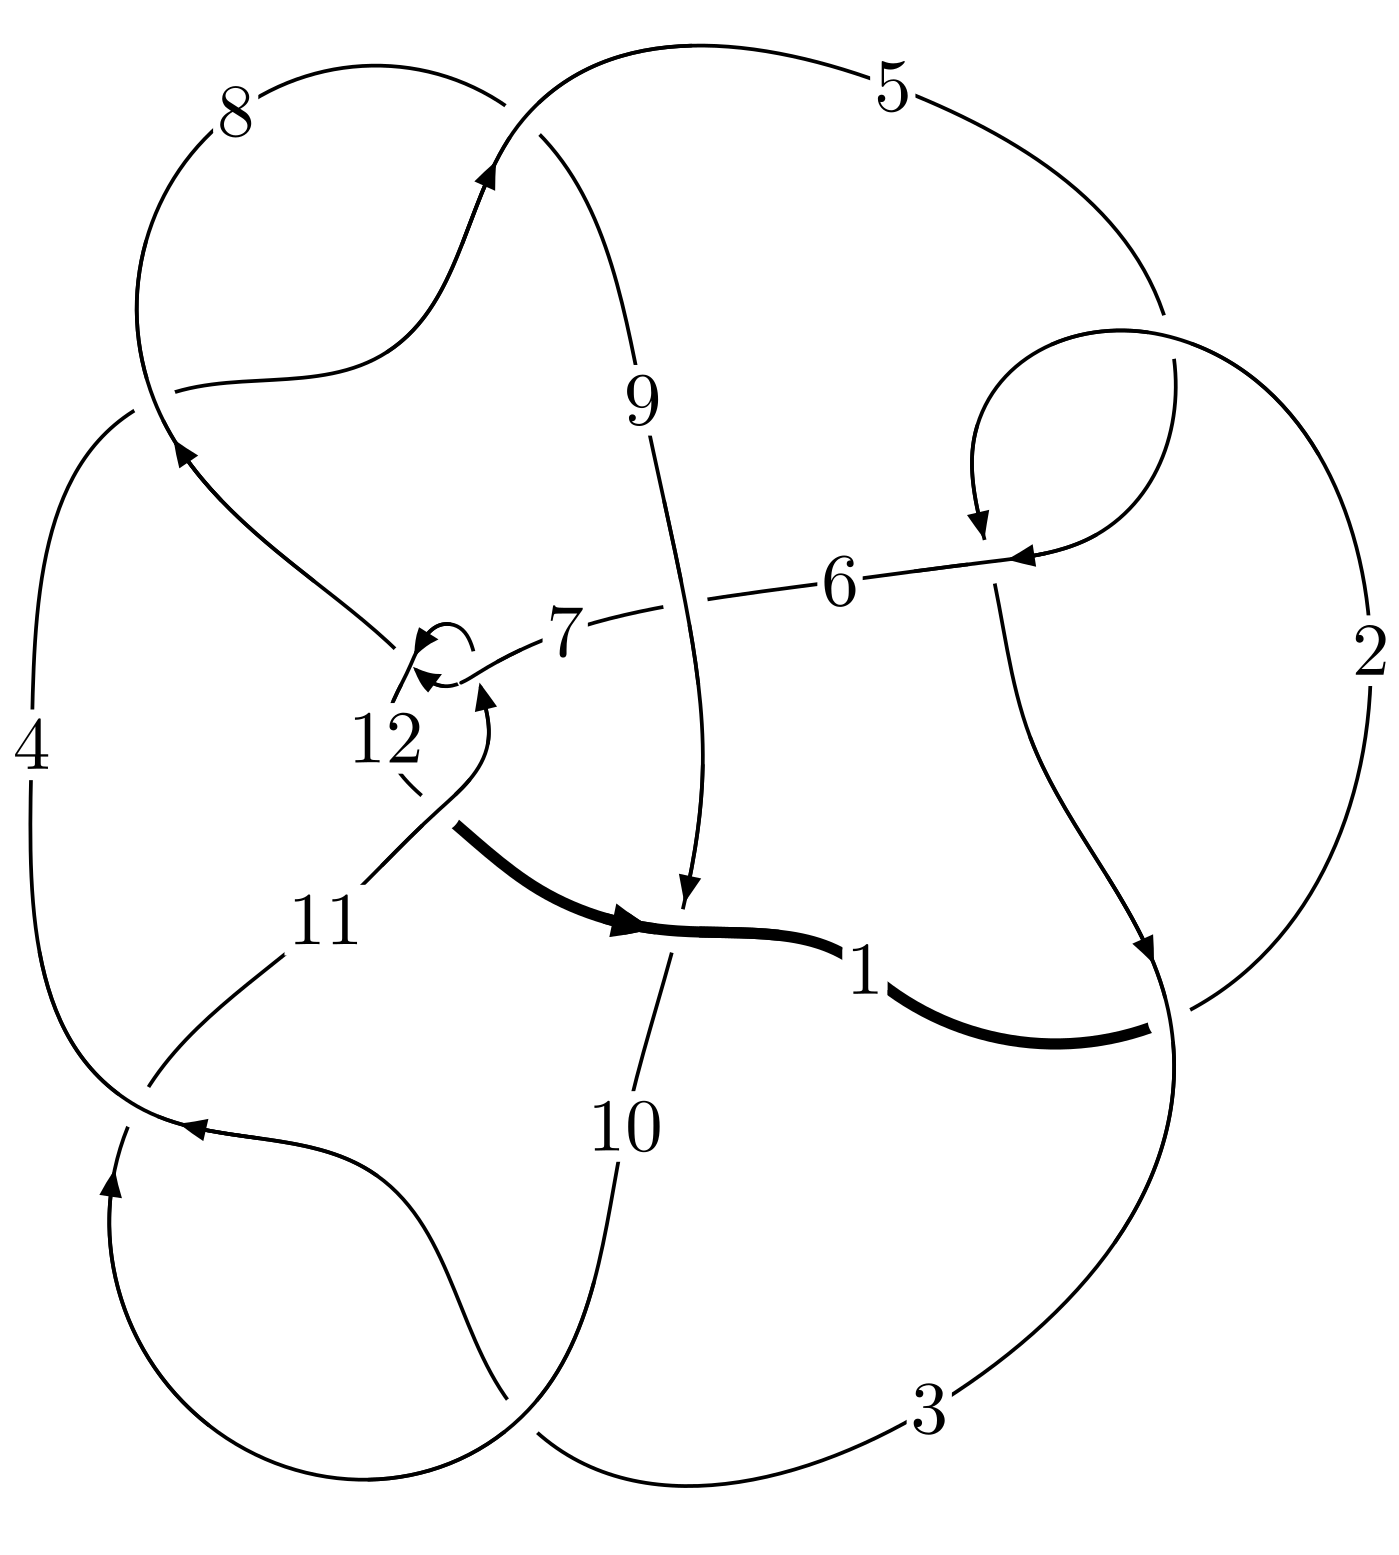
\includegraphics[width=112pt]{../../../GIT/diagram.site/Diagrams/png/1231_12a_0430.png}\\
\ \ \ A knot diagram\footnotemark}&
\allowdisplaybreaks
\textbf{Linearized knot diagam} \\
\cline{2-2}
 &
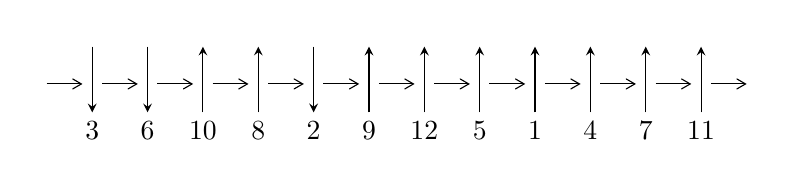
\begin{tikzpicture}[x=20pt, y=17pt]
	% nodes
	\node (C0) at (0, 0) {};
	\node (C1) at (1, 0) {};
	\node (C1U) at (1, +1) {};
	\node (C1D) at (1, -1) {3};

	\node (C2) at (2, 0) {};
	\node (C2U) at (2, +1) {};
	\node (C2D) at (2, -1) {6};

	\node (C3) at (3, 0) {};
	\node (C3U) at (3, +1) {};
	\node (C3D) at (3, -1) {10};

	\node (C4) at (4, 0) {};
	\node (C4U) at (4, +1) {};
	\node (C4D) at (4, -1) {8};

	\node (C5) at (5, 0) {};
	\node (C5U) at (5, +1) {};
	\node (C5D) at (5, -1) {2};

	\node (C6) at (6, 0) {};
	\node (C6U) at (6, +1) {};
	\node (C6D) at (6, -1) {9};

	\node (C7) at (7, 0) {};
	\node (C7U) at (7, +1) {};
	\node (C7D) at (7, -1) {12};

	\node (C8) at (8, 0) {};
	\node (C8U) at (8, +1) {};
	\node (C8D) at (8, -1) {5};

	\node (C9) at (9, 0) {};
	\node (C9U) at (9, +1) {};
	\node (C9D) at (9, -1) {1};

	\node (C10) at (10, 0) {};
	\node (C10U) at (10, +1) {};
	\node (C10D) at (10, -1) {4};

	\node (C11) at (11, 0) {};
	\node (C11U) at (11, +1) {};
	\node (C11D) at (11, -1) {7};

	\node (C12) at (12, 0) {};
	\node (C12U) at (12, +1) {};
	\node (C12D) at (12, -1) {11};
	\node (C13) at (13, 0) {};

	% arrows
	\draw[->,>={angle 60}]
	(C0) edge (C1) (C1) edge (C2) (C2) edge (C3) (C3) edge (C4) (C4) edge (C5) (C5) edge (C6) (C6) edge (C7) (C7) edge (C8) (C8) edge (C9) (C9) edge (C10) (C10) edge (C11) (C11) edge (C12) (C12) edge (C13) ;	\draw[->,>=stealth]
	(C1U) edge (C1D) (C2U) edge (C2D) (C3D) edge (C3U) (C4D) edge (C4U) (C5U) edge (C5D) (C6D) edge (C6U) (C7D) edge (C7U) (C8D) edge (C8U) (C9D) edge (C9U) (C10D) edge (C10U) (C11D) edge (C11U) (C12D) edge (C12U) ;
	\end{tikzpicture} \\
\hhline{~~} \\& 
\textbf{Solving Sequence} \\ \cline{2-2} 
 &
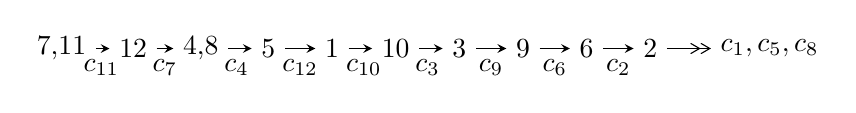
\begin{tikzpicture}[x=23pt, y=7pt]
	% node
	\node (A0) at (-1/8, 0) {7,11};
	\node (A1) at (1, 0) {12};
	\node (A2) at (33/16, 0) {4,8};
	\node (A3) at (25/8, 0) {5};
	\node (A4) at (33/8, 0) {1};
	\node (A5) at (41/8, 0) {10};
	\node (A6) at (49/8, 0) {3};
	\node (A7) at (57/8, 0) {9};
	\node (A8) at (65/8, 0) {6};
	\node (A9) at (73/8, 0) {2};
	\node (C1) at (1/2, -1) {$c_{11}$};
	\node (C2) at (3/2, -1) {$c_{7}$};
	\node (C3) at (21/8, -1) {$c_{4}$};
	\node (C4) at (29/8, -1) {$c_{12}$};
	\node (C5) at (37/8, -1) {$c_{10}$};
	\node (C6) at (45/8, -1) {$c_{3}$};
	\node (C7) at (53/8, -1) {$c_{9}$};
	\node (C8) at (61/8, -1) {$c_{6}$};
	\node (C9) at (69/8, -1) {$c_{2}$};
	\node (A10) at (11, 0) {$c_{1},c_{5},c_{8}$};

	% edge
	\draw[->,>=stealth]	
	(A0) edge (A1) (A1) edge (A2) (A2) edge (A3) (A3) edge (A4) (A4) edge (A5) (A5) edge (A6) (A6) edge (A7) (A7) edge (A8) (A8) edge (A9) ;
	\draw[->>,>={angle 60}]	
	(A9) edge (A10);
\end{tikzpicture} \\ 

\end{tabular} \\

\footnotetext{
The image of knot diagram is generated by the software ``\textbf{Draw programme}" developed by Andrew Bartholomew(\url{http://www.layer8.co.uk/maths/draw/index.htm\#Running-draw}), where we modified some parts for our purpose(\url{https://github.com/CATsTAILs/LinksPainter}).
}\phantom \\ \newline 
\centering \textbf{Ideals for irreducible components\footnotemark of $X_{\text{par}}$} 
 
\begin{align*}
I^u_{1}&=\langle 
-226485 u^{38}-3774546 u^{37}+\cdots+128 b+9282560,\\
\phantom{I^u_{1}}&\phantom{= \langle  }-259737 u^{38}-4524309 u^{37}+\cdots+128 a+21477568,\;3 u^{39}+54 u^{38}+\cdots-3328 u-256\rangle \\
I^u_{2}&=\langle 
-2.26053\times10^{100} a^{15} u^{5}-8.64840\times10^{100} a^{14} u^{5}+\cdots-6.68918\times10^{103} a+2.14623\times10^{103},\\
\phantom{I^u_{2}}&\phantom{= \langle  }- a^{15} u^5-4 a^{14} u^5+\cdots+148 a-22,\;u^6- u^5- u^4+2 u^3- u+1\rangle \\
I^u_{3}&=\langle 
-15 u^{24}+21 u^{23}+\cdots+b-8,\;3 u^{24}-24 u^{23}+\cdots+a-14,\;3 u^{25}-3 u^{24}+\cdots-3 u+1\rangle \\
\\
\end{align*}
\raggedright * 3 irreducible components of $\dim_{\mathbb{C}}=0$, with total 160 representations.\\
\footnotetext{All coefficients of polynomials are rational numbers. But the coefficients are sometimes approximated in decimal forms when there is not enough margin.}
\newpage
\renewcommand{\arraystretch}{1}
\centering \section*{I. $I^u_{1}= \langle -2.26\times10^{5} u^{38}-3.77\times10^{6} u^{37}+\cdots+128 b+9.28\times10^{6},\;-2.60\times10^{5} u^{38}-4.52\times10^{6} u^{37}+\cdots+128 a+2.15\times10^{7},\;3 u^{39}+54 u^{38}+\cdots-3328 u-256 \rangle$}
\flushleft \textbf{(i) Arc colorings}\\
\begin{tabular}{m{7pt} m{180pt} m{7pt} m{180pt} }
\flushright $a_{7}=$&$\begin{pmatrix}0\\u\end{pmatrix}$ \\
\flushright $a_{11}=$&$\begin{pmatrix}1\\0\end{pmatrix}$ \\
\flushright $a_{12}=$&$\begin{pmatrix}1\\- u^2\end{pmatrix}$ \\
\flushright $a_{4}=$&$\begin{pmatrix}2029.20 u^{38}+35346.2 u^{37}+\cdots-2.07355\times10^{6} u-167794.\\1769.41 u^{38}+29488.6 u^{37}+\cdots-948125. u-72520\end{pmatrix}$ \\
\flushright $a_{8}=$&$\begin{pmatrix}u\\- u^3+u\end{pmatrix}$ \\
\flushright $a_{5}=$&$\begin{pmatrix}-331.617 u^{38}-4854.02 u^{37}+\cdots-183199. u-16803.5\\735.914 u^{38}+13795.5 u^{37}+\cdots-1.40161\times10^{6} u-117322\end{pmatrix}$ \\
\flushright $a_{1}=$&$\begin{pmatrix}- u^2+1\\- u^2\end{pmatrix}$ \\
\flushright $a_{10}=$&$\begin{pmatrix}-192.527 u^{38}-3285.52 u^{37}+\cdots+155737 u+12492\\-103.242 u^{38}-1653.28 u^{37}+\cdots+17861 u+1071\end{pmatrix}$ \\
\flushright $a_{3}=$&$\begin{pmatrix}1538.92 u^{38}+26366.7 u^{37}+\cdots-1.44956\times10^{6} u-117071\\491.273 u^{38}+7452.33 u^{37}+\cdots+335799 u+32963\end{pmatrix}$ \\
\flushright $a_{9}=$&$\begin{pmatrix}-12.5508 u^{38}-125.672 u^{37}+\cdots-42277 u-3681\\176.977 u^{38}+3108.84 u^{37}+\cdots-197757 u-16173\end{pmatrix}$ \\
\flushright $a_{6}=$&$\begin{pmatrix}-178.898 u^{38}-3179.23 u^{37}+\cdots+235641. u+19456.5\\-630.586 u^{38}-10679.0 u^{37}+\cdots+481986. u+38544\end{pmatrix}$ \\
\flushright $a_{2}=$&$\begin{pmatrix}271.324 u^{38}+4657.66 u^{37}+\cdots-232931. u-18469\\-293.344 u^{38}-4981.59 u^{37}+\cdots+278367 u+22919\end{pmatrix}$\\&\end{tabular}
\flushleft \textbf{(ii) Obstruction class $= -1$}\\~\\
\flushleft \textbf{(iii) Cusp Shapes $= \frac{1755}{16} u^{38}+\frac{77211}{16} u^{37}+\cdots-2255734 u-193986$}\\~\\
\newpage\renewcommand{\arraystretch}{1}
\flushleft \textbf{(iv) u-Polynomials at the component}\newline \\
\begin{tabular}{m{50pt}|m{274pt}}
Crossings & \hspace{64pt}u-Polynomials at each crossing \\
\hline $$\begin{aligned}c_{1}\end{aligned}$$&$\begin{aligned}
&9(9 u^{39}+114 u^{38}+\cdots+111616 u+4096)
\end{aligned}$\\
\hline $$\begin{aligned}c_{2},c_{5}\end{aligned}$$&$\begin{aligned}
&3(3 u^{39}+48 u^{38}+\cdots-480 u-64)
\end{aligned}$\\
\hline $$\begin{aligned}c_{3},c_{4},c_{8}\\c_{10}\end{aligned}$$&$\begin{aligned}
&u^{39}+2 u^{38}+\cdots+2 u-1
\end{aligned}$\\
\hline $$\begin{aligned}c_{6},c_{9}\end{aligned}$$&$\begin{aligned}
&u^{39}+2 u^{38}+\cdots-33 u-9
\end{aligned}$\\
\hline $$\begin{aligned}c_{7},c_{11}\end{aligned}$$&$\begin{aligned}
&3(3 u^{39}+54 u^{38}+\cdots-3328 u-256)
\end{aligned}$\\
\hline $$\begin{aligned}c_{12}\end{aligned}$$&$\begin{aligned}
&9(9 u^{39}-132 u^{38}+\cdots+262144 u-65536)
\end{aligned}$\\
\hline
\end{tabular}\\~\\
\newpage\renewcommand{\arraystretch}{1}
\flushleft \textbf{(v) Riley Polynomials at the component}\newline \\
\begin{tabular}{m{50pt}|m{274pt}}
Crossings & \hspace{64pt}Riley Polynomials at each crossing \\
\hline $$\begin{aligned}c_{1}\end{aligned}$$&$\begin{aligned}
&81(81 y^{39}+3006 y^{38}+\cdots+5.78080\times10^{9} y-1.67772\times10^{7})
\end{aligned}$\\
\hline $$\begin{aligned}c_{2},c_{5}\end{aligned}$$&$\begin{aligned}
&9(9 y^{39}-114 y^{38}+\cdots+111616 y-4096)
\end{aligned}$\\
\hline $$\begin{aligned}c_{3},c_{4},c_{8}\\c_{10}\end{aligned}$$&$\begin{aligned}
&y^{39}-26 y^{38}+\cdots+52 y^2-1
\end{aligned}$\\
\hline $$\begin{aligned}c_{6},c_{9}\end{aligned}$$&$\begin{aligned}
&y^{39}+36 y^{37}+\cdots+315 y-81
\end{aligned}$\\
\hline $$\begin{aligned}c_{7},c_{11}\end{aligned}$$&$\begin{aligned}
&9(9 y^{39}-132 y^{38}+\cdots+262144 y-65536)
\end{aligned}$\\
\hline $$\begin{aligned}c_{12}\end{aligned}$$&$\begin{aligned}
&81(81 y^{39}+2196 y^{38}+\cdots-6.33508\times10^{10} y-4.29497\times10^{9})
\end{aligned}$\\
\hline
\end{tabular}\\~\\
\newpage\flushleft \textbf{(vi) Complex Volumes and Cusp Shapes}
$$\begin{array}{c|c|c}  
\text{Solutions to }I^u_{1}& \I (\text{vol} + \sqrt{-1}CS) & \text{Cusp shape}\\
 \hline 
\begin{aligned}
u &= -0.227307 + 0.954019 I \\
a &= \phantom{-}0.597619 + 0.748299 I \\
b &= \phantom{-}1.038240 + 0.501550 I\end{aligned}
 & -1.54560 + 5.89382 I & \phantom{-0.000000 } 0 \\ \hline\begin{aligned}
u &= -0.227307 - 0.954019 I \\
a &= \phantom{-}0.597619 - 0.748299 I \\
b &= \phantom{-}1.038240 - 0.501550 I\end{aligned}
 & -1.54560 - 5.89382 I & \phantom{-0.000000 } 0 \\ \hline\begin{aligned}
u &= \phantom{-}0.964633 + 0.040613 I \\
a &= \phantom{-}0.046717 - 0.361973 I \\
b &= -0.131521 + 0.679839 I\end{aligned}
 & \phantom{-}2.24733 + 2.31700 I & \phantom{-0.000000 } 0 \\ \hline\begin{aligned}
u &= \phantom{-}0.964633 - 0.040613 I \\
a &= \phantom{-}0.046717 + 0.361973 I \\
b &= -0.131521 - 0.679839 I\end{aligned}
 & \phantom{-}2.24733 - 2.31700 I & \phantom{-0.000000 } 0 \\ \hline\begin{aligned}
u &= -0.372084 + 0.971347 I \\
a &= \phantom{-}1.033870 + 0.676185 I \\
b &= \phantom{-}1.38505 + 0.53905 I\end{aligned}
 & \phantom{-}5.0495 + 13.3788 I & \phantom{-0.000000 } 0 \\ \hline\begin{aligned}
u &= -0.372084 - 0.971347 I \\
a &= \phantom{-}1.033870 - 0.676185 I \\
b &= \phantom{-}1.38505 - 0.53905 I\end{aligned}
 & \phantom{-}5.0495 - 13.3788 I & \phantom{-0.000000 } 0 \\ \hline\begin{aligned}
u &= -0.366389 + 0.997959 I \\
a &= -0.972711 - 0.584875 I \\
b &= -1.35053 - 0.45887 I\end{aligned}
 & \phantom{-}6.51433 + 7.15268 I & \phantom{-0.000000 } 0 \\ \hline\begin{aligned}
u &= -0.366389 - 0.997959 I \\
a &= -0.972711 + 0.584875 I \\
b &= -1.35053 + 0.45887 I\end{aligned}
 & \phantom{-}6.51433 - 7.15268 I & \phantom{-0.000000 } 0 \\ \hline\begin{aligned}
u &= -0.756872 + 0.753122 I \\
a &= \phantom{-}0.171567 - 0.831323 I \\
b &= \phantom{-}0.450531 - 0.558117 I\end{aligned}
 & -4.96051 - 3.11579 I & \phantom{-0.000000 } 0 \\ \hline\begin{aligned}
u &= -0.756872 - 0.753122 I \\
a &= \phantom{-}0.171567 + 0.831323 I \\
b &= \phantom{-}0.450531 + 0.558117 I\end{aligned}
 & -4.96051 + 3.11579 I & \phantom{-0.000000 } 0\\
 \hline 
 \end{array}$$\newpage$$\begin{array}{c|c|c}  
\text{Solutions to }I^u_{1}& \I (\text{vol} + \sqrt{-1}CS) & \text{Cusp shape}\\
 \hline 
\begin{aligned}
u &= -0.734478 + 0.548916 I \\
a &= \phantom{-}0.333438 + 1.221500 I \\
b &= -0.148939 + 0.692095 I\end{aligned}
 & -1.30683 - 1.81941 I & \phantom{-0.000000 } 0 \\ \hline\begin{aligned}
u &= -0.734478 - 0.548916 I \\
a &= \phantom{-}0.333438 - 1.221500 I \\
b &= -0.148939 - 0.692095 I\end{aligned}
 & -1.30683 + 1.81941 I & \phantom{-0.000000 } 0 \\ \hline\begin{aligned}
u &= -0.928656 + 0.581070 I \\
a &= \phantom{-}0.840210 + 0.897302 I \\
b &= -0.107640 + 0.780975 I\end{aligned}
 & -0.67233 - 2.69467 I & \phantom{-0.000000 } 0 \\ \hline\begin{aligned}
u &= -0.928656 - 0.581070 I \\
a &= \phantom{-}0.840210 - 0.897302 I \\
b &= -0.107640 - 0.780975 I\end{aligned}
 & -0.67233 + 2.69467 I & \phantom{-0.000000 } 0 \\ \hline\begin{aligned}
u &= -0.624790 + 0.647653 I \\
a &= -0.042755 - 1.321680 I \\
b &= \phantom{-}0.185681 - 0.871131 I\end{aligned}
 & -2.58514 + 2.46966 I & \phantom{-0.000000 } 0 \\ \hline\begin{aligned}
u &= -0.624790 - 0.647653 I \\
a &= -0.042755 + 1.321680 I \\
b &= \phantom{-}0.185681 + 0.871131 I\end{aligned}
 & -2.58514 - 2.46966 I & \phantom{-0.000000 } 0 \\ \hline\begin{aligned}
u &= -0.964236 + 0.626940 I \\
a &= -1.015610 - 0.669350 I \\
b &= -0.044585 - 0.877355 I\end{aligned}
 & -1.61000 - 7.43824 I & \phantom{-0.000000 } 0 \\ \hline\begin{aligned}
u &= -0.964236 - 0.626940 I \\
a &= -1.015610 + 0.669350 I \\
b &= -0.044585 + 0.877355 I\end{aligned}
 & -1.61000 + 7.43824 I & \phantom{-0.000000 } 0 \\ \hline\begin{aligned}
u &= -0.927448 + 0.731334 I \\
a &= -0.603265 - 0.055544 I \\
b &= -0.328521 - 0.410615 I\end{aligned}
 & -4.48122 - 2.48257 I & \phantom{-0.000000 } 0 \\ \hline\begin{aligned}
u &= -0.927448 - 0.731334 I \\
a &= -0.603265 + 0.055544 I \\
b &= -0.328521 + 0.410615 I\end{aligned}
 & -4.48122 + 2.48257 I & \phantom{-0.000000 } 0\\
 \hline 
 \end{array}$$\newpage$$\begin{array}{c|c|c}  
\text{Solutions to }I^u_{1}& \I (\text{vol} + \sqrt{-1}CS) & \text{Cusp shape}\\
 \hline 
\begin{aligned}
u &= -0.762524 + 1.065990 I \\
a &= \phantom{-}0.664275 - 0.398822 I \\
b &= \phantom{-}1.098350 - 0.153624 I\end{aligned}
 & \phantom{-}2.59371 - 7.58190 I & \phantom{-0.000000 } 0 \\ \hline\begin{aligned}
u &= -0.762524 - 1.065990 I \\
a &= \phantom{-}0.664275 + 0.398822 I \\
b &= \phantom{-}1.098350 + 0.153624 I\end{aligned}
 & \phantom{-}2.59371 + 7.58190 I & \phantom{-0.000000 } 0 \\ \hline\begin{aligned}
u &= -1.185980 + 0.646068 I \\
a &= \phantom{-}0.29852 + 1.74270 I \\
b &= -1.48593 + 0.60763 I\end{aligned}
 & \phantom{-}7.5533 - 19.2427 I & \phantom{-0.000000 } 0 \\ \hline\begin{aligned}
u &= -1.185980 - 0.646068 I \\
a &= \phantom{-}0.29852 - 1.74270 I \\
b &= -1.48593 - 0.60763 I\end{aligned}
 & \phantom{-}7.5533 + 19.2427 I & \phantom{-0.000000 } 0 \\ \hline\begin{aligned}
u &= \phantom{-}1.353110 + 0.111837 I \\
a &= \phantom{-}0.430891 - 0.154226 I \\
b &= -1.43049 + 0.31053 I\end{aligned}
 & \phantom{-}11.2642 - 9.8374 I & \phantom{-0.000000 } 0 \\ \hline\begin{aligned}
u &= \phantom{-}1.353110 - 0.111837 I \\
a &= \phantom{-}0.430891 + 0.154226 I \\
b &= -1.43049 - 0.31053 I\end{aligned}
 & \phantom{-}11.2642 + 9.8374 I & \phantom{-0.000000 } 0 \\ \hline\begin{aligned}
u &= -1.196030 + 0.650742 I \\
a &= -0.24811 - 1.65622 I \\
b &= \phantom{-}1.45343 - 0.53779 I\end{aligned}
 & \phantom{-}9.0791 - 13.1009 I & \phantom{-0.000000 } 0 \\ \hline\begin{aligned}
u &= -1.196030 - 0.650742 I \\
a &= -0.24811 + 1.65622 I \\
b &= \phantom{-}1.45343 + 0.53779 I\end{aligned}
 & \phantom{-}9.0791 + 13.1009 I & \phantom{-0.000000 } 0 \\ \hline\begin{aligned}
u &= -1.219640 + 0.610960 I \\
a &= \phantom{-}0.47514 + 1.44470 I \\
b &= -1.220300 + 0.570071 I\end{aligned}
 & \phantom{-}1.42407 - 11.55540 I & \phantom{-0.000000 } 0 \\ \hline\begin{aligned}
u &= -1.219640 - 0.610960 I \\
a &= \phantom{-}0.47514 - 1.44470 I \\
b &= -1.220300 - 0.570071 I\end{aligned}
 & \phantom{-}1.42407 + 11.55540 I & \phantom{-0.000000 } 0\\
 \hline 
 \end{array}$$\newpage$$\begin{array}{c|c|c}  
\text{Solutions to }I^u_{1}& \I (\text{vol} + \sqrt{-1}CS) & \text{Cusp shape}\\
 \hline 
\begin{aligned}
u &= \phantom{-}0.618970\phantom{ +0.000000I} \\
a &= \phantom{-}0.307729\phantom{ +0.000000I} \\
b &= -0.308374\phantom{ +0.000000I}\end{aligned}
 & \phantom{-}0.781004\phantom{ +0.000000I} & \phantom{-}13.6700\phantom{ +0.000000I} \\ \hline\begin{aligned}
u &= \phantom{-}1.390700 + 0.097502 I \\
a &= -0.412188 + 0.110529 I \\
b &= \phantom{-}1.40725 - 0.21446 I\end{aligned}
 & \phantom{-}12.91450 - 3.41864 I & \phantom{-0.000000 } 0 \\ \hline\begin{aligned}
u &= \phantom{-}1.390700 - 0.097502 I \\
a &= -0.412188 - 0.110529 I \\
b &= \phantom{-}1.40725 + 0.21446 I\end{aligned}
 & \phantom{-}12.91450 + 3.41864 I & \phantom{-0.000000 } 0 \\ \hline\begin{aligned}
u &= -0.308955 + 0.457236 I \\
a &= \phantom{-}0.037151 + 1.410890 I \\
b &= \phantom{-}0.262188 + 0.589702 I\end{aligned}
 & -1.54604 - 1.25973 I & -0.64918 + 1.74705 I \\ \hline\begin{aligned}
u &= -0.308955 - 0.457236 I \\
a &= \phantom{-}0.037151 - 1.410890 I \\
b &= \phantom{-}0.262188 - 0.589702 I\end{aligned}
 & -1.54604 + 1.25973 I & -0.64918 - 1.74705 I \\ \hline\begin{aligned}
u &= -1.30091 + 0.66769 I \\
a &= -0.221488 - 1.116460 I \\
b &= \phantom{-}1.182050 - 0.297560 I\end{aligned}
 & \phantom{-}7.13968 - 7.57891 I & \phantom{-0.000000 } 0 \\ \hline\begin{aligned}
u &= -1.30091 - 0.66769 I \\
a &= -0.221488 + 1.116460 I \\
b &= \phantom{-}1.182050 + 0.297560 I\end{aligned}
 & \phantom{-}7.13968 + 7.57891 I & \phantom{-0.000000 } 0 \\ \hline\begin{aligned}
u &= -1.14163 + 1.26414 I \\
a &= -0.317136 + 0.372699 I \\
b &= -1.060120 + 0.020872 I\end{aligned}
 & \phantom{-}3.53048 - 0.08358 I & \phantom{-0.000000 } 0 \\ \hline\begin{aligned}
u &= -1.14163 - 1.26414 I \\
a &= -0.317136 - 0.372699 I \\
b &= -1.060120 - 0.020872 I\end{aligned}
 & \phantom{-}3.53048 + 0.08358 I & \phantom{-0.000000 } 0\\
 \hline 
 \end{array}$$\newpage\newpage\renewcommand{\arraystretch}{1}
\centering \section*{II. $I^u_{2}= \langle -2.26\times10^{100} a^{15} u^{5}-8.65\times10^{100} a^{14} u^{5}+\cdots-6.69\times10^{103} a+2.15\times10^{103},\;- a^{15} u^5-4 a^{14} u^5+\cdots+148 a-22,\;u^6- u^5- u^4+2 u^3- u+1 \rangle$}
\flushleft \textbf{(i) Arc colorings}\\
\begin{tabular}{m{7pt} m{180pt} m{7pt} m{180pt} }
\flushright $a_{7}=$&$\begin{pmatrix}0\\u\end{pmatrix}$ \\
\flushright $a_{11}=$&$\begin{pmatrix}1\\0\end{pmatrix}$ \\
\flushright $a_{12}=$&$\begin{pmatrix}1\\- u^2\end{pmatrix}$ \\
\flushright $a_{4}=$&$\begin{pmatrix}a\\0.000688597 a^{15} u^{5}+0.00263445 a^{14} u^{5}+\cdots+2.03764 a-0.653779\end{pmatrix}$ \\
\flushright $a_{8}=$&$\begin{pmatrix}u\\- u^3+u\end{pmatrix}$ \\
\flushright $a_{5}=$&$\begin{pmatrix}0.00313715 a^{15} u^{5}-0.00342694 a^{14} u^{5}+\cdots+1.99577 a-1.83014\\-0.00537123 a^{15} u^{5}-0.00760671 a^{14} u^{5}+\cdots+2.66259 a-2.49184\end{pmatrix}$ \\
\flushright $a_{1}=$&$\begin{pmatrix}- u^2+1\\- u^2\end{pmatrix}$ \\
\flushright $a_{10}=$&$\begin{pmatrix}-0.00523647 a^{15} u^{5}+0.0120349 a^{14} u^{5}+\cdots-0.800101 a+1.31324\\-0.00890304 a^{15} u^{5}+0.0103711 a^{14} u^{5}+\cdots-1.97931 a+2.35126\end{pmatrix}$ \\
\flushright $a_{3}=$&$\begin{pmatrix}-0.0117502 a^{15} u^{5}+0.00137900 a^{14} u^{5}+\cdots-2.84927 a+0.113383\\-0.00974387 a^{15} u^{5}-0.00897497 a^{14} u^{5}+\cdots+0.180125 a-0.421905\end{pmatrix}$ \\
\flushright $a_{9}=$&$\begin{pmatrix}-0.00542664 a^{15} u^{5}-0.00762435 a^{14} u^{5}+\cdots-1.77760 a+0.921213\\-0.0117791 a^{15} u^{5}+0.00831537 a^{14} u^{5}+\cdots-1.12189 a+2.39887\end{pmatrix}$ \\
\flushright $a_{6}=$&$\begin{pmatrix}-0.0112446 a^{15} u^{5}+0.0123645 a^{14} u^{5}+\cdots-0.930856 a+0.943314\\-0.0110795 a^{15} u^{5}+0.0104171 a^{14} u^{5}+\cdots-0.0509322 a+1.85176\end{pmatrix}$ \\
\flushright $a_{2}=$&$\begin{pmatrix}0.00265406 a^{15} u^{5}+0.0238549 a^{14} u^{5}+\cdots-1.23361 a+1.24330\\-0.000235788 a^{15} u^{5}+0.000105668 a^{14} u^{5}+\cdots-0.856035 a-0.131508\end{pmatrix}$\\&\end{tabular}
\flushleft \textbf{(ii) Obstruction class $= -1$}\\~\\
\flushleft \textbf{(iii) Cusp Shapes $= 0.0278817 a^{15} u^{5}-0.0697523 a^{14} u^{5}+\cdots-10.0876 a+4.79726$}\\~\\
\newpage\renewcommand{\arraystretch}{1}
\flushleft \textbf{(iv) u-Polynomials at the component}\newline \\
\begin{tabular}{m{50pt}|m{274pt}}
Crossings & \hspace{64pt}u-Polynomials at each crossing \\
\hline $$\begin{aligned}c_{1}\end{aligned}$$&$\begin{aligned}
&(u^8+3 u^7+7 u^6+10 u^5+11 u^4+10 u^3+6 u^2+4 u+1)^{12}
\end{aligned}$\\
\hline $$\begin{aligned}c_{2},c_{5}\end{aligned}$$&$\begin{aligned}
&(u^8- u^7- u^6+2 u^5+u^4-2 u^3+2 u-1)^{12}
\end{aligned}$\\
\hline $$\begin{aligned}c_{3},c_{4},c_{8}\\c_{10}\end{aligned}$$&$\begin{aligned}
&u^{96}- u^{95}+\cdots-369170 u+47717
\end{aligned}$\\
\hline $$\begin{aligned}c_{6},c_{9}\end{aligned}$$&$\begin{aligned}
&u^{96}+9 u^{95}+\cdots+2219032 u+215401
\end{aligned}$\\
\hline $$\begin{aligned}c_{7},c_{11}\end{aligned}$$&$\begin{aligned}
&(u^6- u^5- u^4+2 u^3- u+1)^{16}
\end{aligned}$\\
\hline $$\begin{aligned}c_{12}\end{aligned}$$&$\begin{aligned}
&(u^6-3 u^5+5 u^4-4 u^3+2 u^2- u+1)^{16}
\end{aligned}$\\
\hline
\end{tabular}\\~\\
\newpage\renewcommand{\arraystretch}{1}
\flushleft \textbf{(v) Riley Polynomials at the component}\newline \\
\begin{tabular}{m{50pt}|m{274pt}}
Crossings & \hspace{64pt}Riley Polynomials at each crossing \\
\hline $$\begin{aligned}c_{1}\end{aligned}$$&$\begin{aligned}
&(y^8+5 y^7+11 y^6+6 y^5-17 y^4-34 y^3-22 y^2-4 y+1)^{12}
\end{aligned}$\\
\hline $$\begin{aligned}c_{2},c_{5}\end{aligned}$$&$\begin{aligned}
&(y^8-3 y^7+7 y^6-10 y^5+11 y^4-10 y^3+6 y^2-4 y+1)^{12}
\end{aligned}$\\
\hline $$\begin{aligned}c_{3},c_{4},c_{8}\\c_{10}\end{aligned}$$&$\begin{aligned}
&y^{96}-81 y^{95}+\cdots-141748367588 y+2276912089
\end{aligned}$\\
\hline $$\begin{aligned}c_{6},c_{9}\end{aligned}$$&$\begin{aligned}
&y^{96}-33 y^{95}+\cdots-549152756700 y+46397590801
\end{aligned}$\\
\hline $$\begin{aligned}c_{7},c_{11}\end{aligned}$$&$\begin{aligned}
&(y^6-3 y^5+5 y^4-4 y^3+2 y^2- y+1)^{16}
\end{aligned}$\\
\hline $$\begin{aligned}c_{12}\end{aligned}$$&$\begin{aligned}
&(y^6+y^5+5 y^4+6 y^2+3 y+1)^{16}
\end{aligned}$\\
\hline
\end{tabular}\\~\\
\newpage\flushleft \textbf{(vi) Complex Volumes and Cusp Shapes}
$$\begin{array}{c|c|c}  
\text{Solutions to }I^u_{2}& \I (\text{vol} + \sqrt{-1}CS) & \text{Cusp shape}\\
 \hline 
\begin{aligned}
u &= -1.002190 + 0.295542 I \\
a &= -0.131228 + 0.966452 I \\
b &= -1.92108 - 0.43745 I\end{aligned}
 & \phantom{-}8.98482 + 1.65419 I & \phantom{-}17.4396 - 2.7737 I \\ \hline\begin{aligned}
u &= -1.002190 + 0.295542 I \\
a &= -0.920754 - 0.485414 I \\
b &= -0.852601 - 0.969355 I\end{aligned}
 & \phantom{-}5.78475 + 0.20693 I & \phantom{-}14.3015 + 0.2834 I \\ \hline\begin{aligned}
u &= -1.002190 + 0.295542 I \\
a &= -0.072117 - 1.131480 I \\
b &= \phantom{-}1.96950 + 0.26401 I\end{aligned}
 & \phantom{-}8.98482 - 3.50280 I & \phantom{-}17.4396 + 4.3622 I \\ \hline\begin{aligned}
u &= -1.002190 + 0.295542 I \\
a &= -0.284942 - 1.232200 I \\
b &= -0.640395 - 0.185153 I\end{aligned}
 & \phantom{-}5.78475 - 2.05554 I & \phantom{-}14.3015 + 1.3050 I \\ \hline\begin{aligned}
u &= -1.002190 + 0.295542 I \\
a &= -0.970327 - 0.812295 I \\
b &= \phantom{-}1.53611 + 0.03337 I\end{aligned}
 & \phantom{-}5.98037 - 0.92430 I & \phantom{-}9.82225 + 0.79423 I \\ \hline\begin{aligned}
u &= -1.002190 + 0.295542 I \\
a &= \phantom{-}1.180110 + 0.543505 I \\
b &= \phantom{-}0.724178 + 1.195600 I\end{aligned}
 & \phantom{-}4.44573 + 5.51923 I & \phantom{-}12.28827 - 4.49994 I \\ \hline\begin{aligned}
u &= -1.002190 + 0.295542 I \\
a &= \phantom{-}1.329820 - 0.337134 I \\
b &= -1.42647 - 0.01572 I\end{aligned}
 & \phantom{-}8.98482 - 3.50280 I & \phantom{-}17.4396 + 4.3622 I \\ \hline\begin{aligned}
u &= -1.002190 + 0.295542 I \\
a &= \phantom{-}0.96287 + 1.09375 I \\
b &= \phantom{-}0.278148 + 0.719400 I\end{aligned}
 & \phantom{-}0.322677 - 0.924305 I & \phantom{-}7.85268 + 0.79423 I \\ \hline\begin{aligned}
u &= -1.002190 + 0.295542 I \\
a &= -1.49099 + 0.08573 I \\
b &= \phantom{-}1.47063 + 0.04551 I\end{aligned}
 & \phantom{-}8.98482 + 1.65419 I & \phantom{-}17.4396 - 2.7737 I \\ \hline\begin{aligned}
u &= -1.002190 + 0.295542 I \\
a &= \phantom{-}0.38868 + 1.53392 I \\
b &= \phantom{-}0.450129 + 0.033041 I\end{aligned}
 & \phantom{-}4.44573 - 7.36784 I & \phantom{-}12.28827 + 6.08840 I\\
 \hline 
 \end{array}$$\newpage$$\begin{array}{c|c|c}  
\text{Solutions to }I^u_{2}& \I (\text{vol} + \sqrt{-1}CS) & \text{Cusp shape}\\
 \hline 
\begin{aligned}
u &= -1.002190 + 0.295542 I \\
a &= \phantom{-}0.188568 - 0.080838 I \\
b &= -1.337560 - 0.341469 I\end{aligned}
 & \phantom{-}5.98037 - 0.92430 I & \phantom{-}9.82225 + 0.79423 I \\ \hline\begin{aligned}
u &= -1.002190 + 0.295542 I \\
a &= -1.18748 - 1.49401 I \\
b &= \phantom{-}1.324260 - 0.484048 I\end{aligned}
 & \phantom{-}5.78475 - 2.05554 I & \phantom{-}14.3015 + 1.3050 I \\ \hline\begin{aligned}
u &= -1.002190 + 0.295542 I \\
a &= \phantom{-}1.24714 + 1.57460 I \\
b &= -1.23357 + 0.71721 I\end{aligned}
 & \phantom{-}4.44573 - 7.36784 I & \phantom{-}12.28827 + 6.08840 I \\ \hline\begin{aligned}
u &= -1.002190 + 0.295542 I \\
a &= \phantom{-}1.34882 + 1.54727 I \\
b &= -0.865270 + 0.191673 I\end{aligned}
 & \phantom{-}0.322677 - 0.924305 I & \phantom{-}7.85268 + 0.79423 I \\ \hline\begin{aligned}
u &= -1.002190 + 0.295542 I \\
a &= -1.58649 - 1.33501 I \\
b &= \phantom{-}1.179490 + 0.070105 I\end{aligned}
 & \phantom{-}5.78475 + 0.20693 I & \phantom{-}14.3015 + 0.2834 I \\ \hline\begin{aligned}
u &= -1.002190 + 0.295542 I \\
a &= \phantom{-}1.68445 + 1.48950 I \\
b &= -1.083740 - 0.172180 I\end{aligned}
 & \phantom{-}4.44573 + 5.51923 I & \phantom{-}12.28827 - 4.49994 I \\ \hline\begin{aligned}
u &= -1.002190 - 0.295542 I \\
a &= -0.131228 - 0.966452 I \\
b &= -1.92108 + 0.43745 I\end{aligned}
 & \phantom{-}8.98482 - 1.65419 I & \phantom{-}17.4396 + 2.7737 I \\ \hline\begin{aligned}
u &= -1.002190 - 0.295542 I \\
a &= -0.920754 + 0.485414 I \\
b &= -0.852601 + 0.969355 I\end{aligned}
 & \phantom{-}5.78475 - 0.20693 I & \phantom{-}14.3015 - 0.2834 I \\ \hline\begin{aligned}
u &= -1.002190 - 0.295542 I \\
a &= -0.072117 + 1.131480 I \\
b &= \phantom{-}1.96950 - 0.26401 I\end{aligned}
 & \phantom{-}8.98482 + 3.50280 I & \phantom{-}17.4396 - 4.3622 I \\ \hline\begin{aligned}
u &= -1.002190 - 0.295542 I \\
a &= -0.284942 + 1.232200 I \\
b &= -0.640395 + 0.185153 I\end{aligned}
 & \phantom{-}5.78475 + 2.05554 I & \phantom{-}14.3015 - 1.3050 I\\
 \hline 
 \end{array}$$\newpage$$\begin{array}{c|c|c}  
\text{Solutions to }I^u_{2}& \I (\text{vol} + \sqrt{-1}CS) & \text{Cusp shape}\\
 \hline 
\begin{aligned}
u &= -1.002190 - 0.295542 I \\
a &= -0.970327 + 0.812295 I \\
b &= \phantom{-}1.53611 - 0.03337 I\end{aligned}
 & \phantom{-}5.98037 + 0.92430 I & \phantom{-}9.82225 - 0.79423 I \\ \hline\begin{aligned}
u &= -1.002190 - 0.295542 I \\
a &= \phantom{-}1.180110 - 0.543505 I \\
b &= \phantom{-}0.724178 - 1.195600 I\end{aligned}
 & \phantom{-}4.44573 - 5.51923 I & \phantom{-}12.28827 + 4.49994 I \\ \hline\begin{aligned}
u &= -1.002190 - 0.295542 I \\
a &= \phantom{-}1.329820 + 0.337134 I \\
b &= -1.42647 + 0.01572 I\end{aligned}
 & \phantom{-}8.98482 + 3.50280 I & \phantom{-}17.4396 - 4.3622 I \\ \hline\begin{aligned}
u &= -1.002190 - 0.295542 I \\
a &= \phantom{-}0.96287 - 1.09375 I \\
b &= \phantom{-}0.278148 - 0.719400 I\end{aligned}
 & \phantom{-}0.322677 + 0.924305 I & \phantom{-}7.85268 - 0.79423 I \\ \hline\begin{aligned}
u &= -1.002190 - 0.295542 I \\
a &= -1.49099 - 0.08573 I \\
b &= \phantom{-}1.47063 - 0.04551 I\end{aligned}
 & \phantom{-}8.98482 - 1.65419 I & \phantom{-}17.4396 + 2.7737 I \\ \hline\begin{aligned}
u &= -1.002190 - 0.295542 I \\
a &= \phantom{-}0.38868 - 1.53392 I \\
b &= \phantom{-}0.450129 - 0.033041 I\end{aligned}
 & \phantom{-}4.44573 + 7.36784 I & \phantom{-}12.28827 - 6.08840 I \\ \hline\begin{aligned}
u &= -1.002190 - 0.295542 I \\
a &= \phantom{-}0.188568 + 0.080838 I \\
b &= -1.337560 + 0.341469 I\end{aligned}
 & \phantom{-}5.98037 + 0.92430 I & \phantom{-}9.82225 - 0.79423 I \\ \hline\begin{aligned}
u &= -1.002190 - 0.295542 I \\
a &= -1.18748 + 1.49401 I \\
b &= \phantom{-}1.324260 + 0.484048 I\end{aligned}
 & \phantom{-}5.78475 + 2.05554 I & \phantom{-}14.3015 - 1.3050 I \\ \hline\begin{aligned}
u &= -1.002190 - 0.295542 I \\
a &= \phantom{-}1.24714 - 1.57460 I \\
b &= -1.23357 - 0.71721 I\end{aligned}
 & \phantom{-}4.44573 + 7.36784 I & \phantom{-}12.28827 - 6.08840 I \\ \hline\begin{aligned}
u &= -1.002190 - 0.295542 I \\
a &= \phantom{-}1.34882 - 1.54727 I \\
b &= -0.865270 - 0.191673 I\end{aligned}
 & \phantom{-}0.322677 + 0.924305 I & \phantom{-}7.85268 - 0.79423 I\\
 \hline 
 \end{array}$$\newpage$$\begin{array}{c|c|c}  
\text{Solutions to }I^u_{2}& \I (\text{vol} + \sqrt{-1}CS) & \text{Cusp shape}\\
 \hline 
\begin{aligned}
u &= -1.002190 - 0.295542 I \\
a &= -1.58649 + 1.33501 I \\
b &= \phantom{-}1.179490 - 0.070105 I\end{aligned}
 & \phantom{-}5.78475 - 0.20693 I & \phantom{-}14.3015 - 0.2834 I \\ \hline\begin{aligned}
u &= -1.002190 - 0.295542 I \\
a &= \phantom{-}1.68445 - 1.48950 I \\
b &= -1.083740 + 0.172180 I\end{aligned}
 & \phantom{-}4.44573 - 5.51923 I & \phantom{-}12.28827 + 4.49994 I \\ \hline\begin{aligned}
u &= \phantom{-}0.428243 + 0.664531 I \\
a &= \phantom{-}0.338368 - 0.856179 I \\
b &= \phantom{-}1.220680 - 0.477407 I\end{aligned}
 & \phantom{-}0.66452 - 7.36784 I & \phantom{-}4.85484 + 6.08840 I \\ \hline\begin{aligned}
u &= \phantom{-}0.428243 + 0.664531 I \\
a &= -0.495098 + 0.691509 I \\
b &= -1.206330 + 0.367263 I\end{aligned}
 & \phantom{-}2.00354 - 2.05554 I & \phantom{-}6.86806 + 1.30502 I \\ \hline\begin{aligned}
u &= \phantom{-}0.428243 + 0.664531 I \\
a &= \phantom{-}0.714452 - 0.421331 I \\
b &= -0.217102 + 0.071087 I\end{aligned}
 & \phantom{-}2.00354 + 0.20693 I & \phantom{-}6.86806 + 0.28344 I \\ \hline\begin{aligned}
u &= \phantom{-}0.428243 + 0.664531 I \\
a &= -0.512773 - 0.573888 I \\
b &= -1.044990 - 0.150675 I\end{aligned}
 & \phantom{-}2.00354 + 0.20693 I & \phantom{-}6.86806 + 0.28344 I \\ \hline\begin{aligned}
u &= \phantom{-}0.428243 + 0.664531 I \\
a &= \phantom{-}0.475180 + 1.143100 I \\
b &= \phantom{-}1.061230 + 0.489637 I\end{aligned}
 & \phantom{-}0.66452 + 5.51923 I & \phantom{-}4.85484 - 4.49994 I \\ \hline\begin{aligned}
u &= \phantom{-}0.428243 + 0.664531 I \\
a &= -0.691630 - 0.012427 I \\
b &= \phantom{-}0.370476 - 0.414858 I\end{aligned}
 & \phantom{-}0.66452 + 5.51923 I & \phantom{-}4.85484 - 4.49994 I \\ \hline\begin{aligned}
u &= \phantom{-}0.428243 + 0.664531 I \\
a &= -1.290680 + 0.422211 I \\
b &= -1.230390 + 0.212303 I\end{aligned}
 & \phantom{-}2.19916 - 0.92430 I & \phantom{-}2.38882 + 0.79423 I \\ \hline\begin{aligned}
u &= \phantom{-}0.428243 + 0.664531 I \\
a &= -0.021113 - 0.454124 I \\
b &= \phantom{-}0.928150 - 0.448492 I\end{aligned}
 & -3.45853 - 0.92430 I & \phantom{-}0.419245 + 0.794226 I\\
 \hline 
 \end{array}$$\newpage$$\begin{array}{c|c|c}  
\text{Solutions to }I^u_{2}& \I (\text{vol} + \sqrt{-1}CS) & \text{Cusp shape}\\
 \hline 
\begin{aligned}
u &= \phantom{-}0.428243 + 0.664531 I \\
a &= -0.45184 + 1.50268 I \\
b &= \phantom{-}0.445858 + 0.853680 I\end{aligned}
 & -3.45853 - 0.92430 I & \phantom{-}0.419245 + 0.794226 I \\ \hline\begin{aligned}
u &= \phantom{-}0.428243 + 0.664531 I \\
a &= -1.42972 + 0.79073 I \\
b &= -1.201220 - 0.073274 I\end{aligned}
 & \phantom{-}5.20361 - 3.50280 I & \phantom{-}10.00621 + 4.36218 I \\ \hline\begin{aligned}
u &= \phantom{-}0.428243 + 0.664531 I \\
a &= \phantom{-}1.45063 - 0.77681 I \\
b &= \phantom{-}0.765736 - 0.349328 I\end{aligned}
 & \phantom{-}2.19916 - 0.92430 I & \phantom{-}2.38882 + 0.79423 I \\ \hline\begin{aligned}
u &= \phantom{-}0.428243 + 0.664531 I \\
a &= \phantom{-}1.48375 - 0.73194 I \\
b &= \phantom{-}1.090890 + 0.140025 I\end{aligned}
 & \phantom{-}5.20361 + 1.65419 I & \phantom{-}10.00621 - 2.77373 I \\ \hline\begin{aligned}
u &= \phantom{-}0.428243 + 0.664531 I \\
a &= \phantom{-}1.10763 - 1.50141 I \\
b &= \phantom{-}0.103004 - 0.985223 I\end{aligned}
 & \phantom{-}2.00354 - 2.05554 I & \phantom{-}6.86806 + 1.30502 I \\ \hline\begin{aligned}
u &= \phantom{-}0.428243 + 0.664531 I \\
a &= -1.04266 + 1.76681 I \\
b &= \phantom{-}0.022518 + 1.191450 I\end{aligned}
 & \phantom{-}0.66452 - 7.36784 I & \phantom{-}4.85484 + 6.08840 I \\ \hline\begin{aligned}
u &= \phantom{-}0.428243 + 0.664531 I \\
a &= -2.01816 + 0.39141 I \\
b &= -1.42014 + 0.57718 I\end{aligned}
 & \phantom{-}5.20361 + 1.65419 I & \phantom{-}10.00621 - 2.77373 I \\ \hline\begin{aligned}
u &= \phantom{-}0.428243 + 0.664531 I \\
a &= \phantom{-}2.03871 - 0.61553 I \\
b &= \phantom{-}1.31381 - 0.70782 I\end{aligned}
 & \phantom{-}5.20361 - 3.50280 I & \phantom{-}10.00621 + 4.36218 I \\ \hline\begin{aligned}
u &= \phantom{-}0.428243 - 0.664531 I \\
a &= \phantom{-}0.338368 + 0.856179 I \\
b &= \phantom{-}1.220680 + 0.477407 I\end{aligned}
 & \phantom{-}0.66452 + 7.36784 I & \phantom{-}4.85484 - 6.08840 I \\ \hline\begin{aligned}
u &= \phantom{-}0.428243 - 0.664531 I \\
a &= -0.495098 - 0.691509 I \\
b &= -1.206330 - 0.367263 I\end{aligned}
 & \phantom{-}2.00354 + 2.05554 I & \phantom{-}6.86806 - 1.30502 I\\
 \hline 
 \end{array}$$\newpage$$\begin{array}{c|c|c}  
\text{Solutions to }I^u_{2}& \I (\text{vol} + \sqrt{-1}CS) & \text{Cusp shape}\\
 \hline 
\begin{aligned}
u &= \phantom{-}0.428243 - 0.664531 I \\
a &= \phantom{-}0.714452 + 0.421331 I \\
b &= -0.217102 - 0.071087 I\end{aligned}
 & \phantom{-}2.00354 - 0.20693 I & \phantom{-}6.86806 - 0.28344 I \\ \hline\begin{aligned}
u &= \phantom{-}0.428243 - 0.664531 I \\
a &= -0.512773 + 0.573888 I \\
b &= -1.044990 + 0.150675 I\end{aligned}
 & \phantom{-}2.00354 - 0.20693 I & \phantom{-}6.86806 - 0.28344 I \\ \hline\begin{aligned}
u &= \phantom{-}0.428243 - 0.664531 I \\
a &= \phantom{-}0.475180 - 1.143100 I \\
b &= \phantom{-}1.061230 - 0.489637 I\end{aligned}
 & \phantom{-}0.66452 - 5.51923 I & \phantom{-}4.85484 + 4.49994 I \\ \hline\begin{aligned}
u &= \phantom{-}0.428243 - 0.664531 I \\
a &= -0.691630 + 0.012427 I \\
b &= \phantom{-}0.370476 + 0.414858 I\end{aligned}
 & \phantom{-}0.66452 - 5.51923 I & \phantom{-}4.85484 + 4.49994 I \\ \hline\begin{aligned}
u &= \phantom{-}0.428243 - 0.664531 I \\
a &= -1.290680 - 0.422211 I \\
b &= -1.230390 - 0.212303 I\end{aligned}
 & \phantom{-}2.19916 + 0.92430 I & \phantom{-}2.38882 - 0.79423 I \\ \hline\begin{aligned}
u &= \phantom{-}0.428243 - 0.664531 I \\
a &= -0.021113 + 0.454124 I \\
b &= \phantom{-}0.928150 + 0.448492 I\end{aligned}
 & -3.45853 + 0.92430 I & \phantom{-}0.419245 - 0.794226 I \\ \hline\begin{aligned}
u &= \phantom{-}0.428243 - 0.664531 I \\
a &= -0.45184 - 1.50268 I \\
b &= \phantom{-}0.445858 - 0.853680 I\end{aligned}
 & -3.45853 + 0.92430 I & \phantom{-}0.419245 - 0.794226 I \\ \hline\begin{aligned}
u &= \phantom{-}0.428243 - 0.664531 I \\
a &= -1.42972 - 0.79073 I \\
b &= -1.201220 + 0.073274 I\end{aligned}
 & \phantom{-}5.20361 + 3.50280 I & \phantom{-}10.00621 - 4.36218 I \\ \hline\begin{aligned}
u &= \phantom{-}0.428243 - 0.664531 I \\
a &= \phantom{-}1.45063 + 0.77681 I \\
b &= \phantom{-}0.765736 + 0.349328 I\end{aligned}
 & \phantom{-}2.19916 + 0.92430 I & \phantom{-}2.38882 - 0.79423 I \\ \hline\begin{aligned}
u &= \phantom{-}0.428243 - 0.664531 I \\
a &= \phantom{-}1.48375 + 0.73194 I \\
b &= \phantom{-}1.090890 - 0.140025 I\end{aligned}
 & \phantom{-}5.20361 - 1.65419 I & \phantom{-}10.00621 + 2.77373 I\\
 \hline 
 \end{array}$$\newpage$$\begin{array}{c|c|c}  
\text{Solutions to }I^u_{2}& \I (\text{vol} + \sqrt{-1}CS) & \text{Cusp shape}\\
 \hline 
\begin{aligned}
u &= \phantom{-}0.428243 - 0.664531 I \\
a &= \phantom{-}1.10763 + 1.50141 I \\
b &= \phantom{-}0.103004 + 0.985223 I\end{aligned}
 & \phantom{-}2.00354 + 2.05554 I & \phantom{-}6.86806 - 1.30502 I \\ \hline\begin{aligned}
u &= \phantom{-}0.428243 - 0.664531 I \\
a &= -1.04266 - 1.76681 I \\
b &= \phantom{-}0.022518 - 1.191450 I\end{aligned}
 & \phantom{-}0.66452 + 7.36784 I & \phantom{-}4.85484 - 6.08840 I \\ \hline\begin{aligned}
u &= \phantom{-}0.428243 - 0.664531 I \\
a &= -2.01816 - 0.39141 I \\
b &= -1.42014 - 0.57718 I\end{aligned}
 & \phantom{-}5.20361 - 1.65419 I & \phantom{-}10.00621 + 2.77373 I \\ \hline\begin{aligned}
u &= \phantom{-}0.428243 - 0.664531 I \\
a &= \phantom{-}2.03871 + 0.61553 I \\
b &= \phantom{-}1.31381 + 0.70782 I\end{aligned}
 & \phantom{-}5.20361 + 3.50280 I & \phantom{-}10.00621 - 4.36218 I \\ \hline\begin{aligned}
u &= \phantom{-}1.073950 + 0.558752 I \\
a &= -0.664094 + 0.668228 I \\
b &= -0.295117 + 1.104200 I\end{aligned}
 & -1.56793 + 5.69302 I & \phantom{-}4.13596 - 5.51057 I \\ \hline\begin{aligned}
u &= \phantom{-}1.073950 + 0.558752 I \\
a &= -0.193047 + 1.198190 I \\
b &= \phantom{-}1.315860 + 0.064316 I\end{aligned}
 & \phantom{-}3.89415 + 4.56179 I & \phantom{-}10.58478 - 4.99978 I \\ \hline\begin{aligned}
u &= \phantom{-}1.073950 + 0.558752 I \\
a &= -0.111947 - 0.724388 I \\
b &= \phantom{-}0.101611 - 0.435249 I\end{aligned}
 & \phantom{-}3.89415 + 4.56179 I & \phantom{-}10.58478 - 4.99978 I \\ \hline\begin{aligned}
u &= \phantom{-}1.073950 + 0.558752 I \\
a &= \phantom{-}0.081352 - 0.699474 I \\
b &= -1.105270 + 0.161393 I\end{aligned}
 & \phantom{-}2.55512 - 0.75052 I & \phantom{-}8.57155 - 0.21640 I \\ \hline\begin{aligned}
u &= \phantom{-}1.073950 + 0.558752 I \\
a &= \phantom{-}0.717274 - 1.217360 I \\
b &= -0.226353 - 1.304860 I\end{aligned}
 & \phantom{-}3.89415 + 6.82425 I & \phantom{-}10.58478 - 6.02136 I \\ \hline\begin{aligned}
u &= \phantom{-}1.073950 + 0.558752 I \\
a &= -0.93532 + 1.14301 I \\
b &= \phantom{-}0.08300 + 1.50716 I\end{aligned}
 & \phantom{-}2.55512 + 12.13660 I & \phantom{-}8.57155 - 10.80474 I\\
 \hline 
 \end{array}$$\newpage$$\begin{array}{c|c|c}  
\text{Solutions to }I^u_{2}& \I (\text{vol} + \sqrt{-1}CS) & \text{Cusp shape}\\
 \hline 
\begin{aligned}
u &= \phantom{-}1.073950 + 0.558752 I \\
a &= \phantom{-}0.88186 - 1.26823 I \\
b &= -1.177270 - 0.338145 I\end{aligned}
 & -1.56793 + 5.69302 I & \phantom{-}4.13596 - 5.51057 I \\ \hline\begin{aligned}
u &= \phantom{-}1.073950 + 0.558752 I \\
a &= \phantom{-}0.270195 + 0.166091 I \\
b &= -0.506146 + 0.241762 I\end{aligned}
 & \phantom{-}2.55512 - 0.75052 I & \phantom{-}8.57155 - 0.21640 I \\ \hline\begin{aligned}
u &= \phantom{-}1.073950 + 0.558752 I \\
a &= \phantom{-}0.10508 - 1.69146 I \\
b &= -0.867965 - 0.637909 I\end{aligned}
 & \phantom{-}4.08977 + 5.69302 I & \phantom{-}6.10554 - 5.51057 I \\ \hline\begin{aligned}
u &= \phantom{-}1.073950 + 0.558752 I \\
a &= -0.17872 + 1.89437 I \\
b &= \phantom{-}1.36589 + 0.37885 I\end{aligned}
 & \phantom{-}4.08977 + 5.69302 I & \phantom{-}6.10554 - 5.51057 I \\ \hline\begin{aligned}
u &= \phantom{-}1.073950 + 0.558752 I \\
a &= -0.78717 + 1.77649 I \\
b &= \phantom{-}1.343660 + 0.357004 I\end{aligned}
 & \phantom{-}3.89415 + 6.82425 I & \phantom{-}10.58478 - 6.02136 I \\ \hline\begin{aligned}
u &= \phantom{-}1.073950 + 0.558752 I \\
a &= \phantom{-}1.00771 - 1.77771 I \\
b &= -1.338020 - 0.418979 I\end{aligned}
 & \phantom{-}2.55512 + 12.13660 I & \phantom{-}8.57155 - 10.80474 I \\ \hline\begin{aligned}
u &= \phantom{-}1.073950 + 0.558752 I \\
a &= -0.11963 + 2.06380 I \\
b &= \phantom{-}1.62571 + 0.82625 I\end{aligned}
 & \phantom{-}7.09422 + 3.11453 I & \phantom{-}13.72292 - 1.94261 I \\ \hline\begin{aligned}
u &= \phantom{-}1.073950 + 0.558752 I \\
a &= \phantom{-}0.23274 - 2.06246 I \\
b &= -1.50878 - 0.98090 I\end{aligned}
 & \phantom{-}7.09422 + 8.27152 I & \phantom{-}13.7229 - 9.0785 I \\ \hline\begin{aligned}
u &= \phantom{-}1.073950 + 0.558752 I \\
a &= -0.22467 - 2.13523 I \\
b &= -1.091960 - 0.083854 I\end{aligned}
 & \phantom{-}7.09422 + 3.11453 I & \phantom{-}13.72292 - 1.94261 I \\ \hline\begin{aligned}
u &= \phantom{-}1.073950 + 0.558752 I \\
a &= \phantom{-}0.07723 + 2.22849 I \\
b &= \phantom{-}1.207190 + 0.117716 I\end{aligned}
 & \phantom{-}7.09422 + 8.27152 I & \phantom{-}13.7229 - 9.0785 I\\
 \hline 
 \end{array}$$\newpage$$\begin{array}{c|c|c}  
\text{Solutions to }I^u_{2}& \I (\text{vol} + \sqrt{-1}CS) & \text{Cusp shape}\\
 \hline 
\begin{aligned}
u &= \phantom{-}1.073950 - 0.558752 I \\
a &= -0.664094 - 0.668228 I \\
b &= -0.295117 - 1.104200 I\end{aligned}
 & -1.56793 - 5.69302 I & \phantom{-}4.13596 + 5.51057 I \\ \hline\begin{aligned}
u &= \phantom{-}1.073950 - 0.558752 I \\
a &= -0.193047 - 1.198190 I \\
b &= \phantom{-}1.315860 - 0.064316 I\end{aligned}
 & \phantom{-}3.89415 - 4.56179 I & \phantom{-}10.58478 + 4.99978 I \\ \hline\begin{aligned}
u &= \phantom{-}1.073950 - 0.558752 I \\
a &= -0.111947 + 0.724388 I \\
b &= \phantom{-}0.101611 + 0.435249 I\end{aligned}
 & \phantom{-}3.89415 - 4.56179 I & \phantom{-}10.58478 + 4.99978 I \\ \hline\begin{aligned}
u &= \phantom{-}1.073950 - 0.558752 I \\
a &= \phantom{-}0.081352 + 0.699474 I \\
b &= -1.105270 - 0.161393 I\end{aligned}
 & \phantom{-}2.55512 + 0.75052 I & \phantom{-}8.57155 + 0.21640 I \\ \hline\begin{aligned}
u &= \phantom{-}1.073950 - 0.558752 I \\
a &= \phantom{-}0.717274 + 1.217360 I \\
b &= -0.226353 + 1.304860 I\end{aligned}
 & \phantom{-}3.89415 - 6.82425 I & \phantom{-}10.58478 + 6.02136 I \\ \hline\begin{aligned}
u &= \phantom{-}1.073950 - 0.558752 I \\
a &= -0.93532 - 1.14301 I \\
b &= \phantom{-}0.08300 - 1.50716 I\end{aligned}
 & \phantom{-}2.55512 - 12.13660 I & \phantom{-}8.57155 + 10.80474 I \\ \hline\begin{aligned}
u &= \phantom{-}1.073950 - 0.558752 I \\
a &= \phantom{-}0.88186 + 1.26823 I \\
b &= -1.177270 + 0.338145 I\end{aligned}
 & -1.56793 - 5.69302 I & \phantom{-}4.13596 + 5.51057 I \\ \hline\begin{aligned}
u &= \phantom{-}1.073950 - 0.558752 I \\
a &= \phantom{-}0.270195 - 0.166091 I \\
b &= -0.506146 - 0.241762 I\end{aligned}
 & \phantom{-}2.55512 + 0.75052 I & \phantom{-}8.57155 + 0.21640 I \\ \hline\begin{aligned}
u &= \phantom{-}1.073950 - 0.558752 I \\
a &= \phantom{-}0.10508 + 1.69146 I \\
b &= -0.867965 + 0.637909 I\end{aligned}
 & \phantom{-}4.08977 - 5.69302 I & \phantom{-}6.10554 + 5.51057 I \\ \hline\begin{aligned}
u &= \phantom{-}1.073950 - 0.558752 I \\
a &= -0.17872 - 1.89437 I \\
b &= \phantom{-}1.36589 - 0.37885 I\end{aligned}
 & \phantom{-}4.08977 - 5.69302 I & \phantom{-}6.10554 + 5.51057 I\\
 \hline 
 \end{array}$$\newpage$$\begin{array}{c|c|c}  
\text{Solutions to }I^u_{2}& \I (\text{vol} + \sqrt{-1}CS) & \text{Cusp shape}\\
 \hline 
\begin{aligned}
u &= \phantom{-}1.073950 - 0.558752 I \\
a &= -0.78717 - 1.77649 I \\
b &= \phantom{-}1.343660 - 0.357004 I\end{aligned}
 & \phantom{-}3.89415 - 6.82425 I & \phantom{-}10.58478 + 6.02136 I \\ \hline\begin{aligned}
u &= \phantom{-}1.073950 - 0.558752 I \\
a &= \phantom{-}1.00771 + 1.77771 I \\
b &= -1.338020 + 0.418979 I\end{aligned}
 & \phantom{-}2.55512 - 12.13660 I & \phantom{-}8.57155 + 10.80474 I \\ \hline\begin{aligned}
u &= \phantom{-}1.073950 - 0.558752 I \\
a &= -0.11963 - 2.06380 I \\
b &= \phantom{-}1.62571 - 0.82625 I\end{aligned}
 & \phantom{-}7.09422 - 3.11453 I & \phantom{-}13.72292 + 1.94261 I \\ \hline\begin{aligned}
u &= \phantom{-}1.073950 - 0.558752 I \\
a &= \phantom{-}0.23274 + 2.06246 I \\
b &= -1.50878 + 0.98090 I\end{aligned}
 & \phantom{-}7.09422 - 8.27152 I & \phantom{-}13.7229 + 9.0785 I \\ \hline\begin{aligned}
u &= \phantom{-}1.073950 - 0.558752 I \\
a &= -0.22467 + 2.13523 I \\
b &= -1.091960 + 0.083854 I\end{aligned}
 & \phantom{-}7.09422 - 3.11453 I & \phantom{-}13.72292 + 1.94261 I \\ \hline\begin{aligned}
u &= \phantom{-}1.073950 - 0.558752 I \\
a &= \phantom{-}0.07723 - 2.22849 I \\
b &= \phantom{-}1.207190 - 0.117716 I\end{aligned}
 & \phantom{-}7.09422 - 8.27152 I & \phantom{-}13.7229 + 9.0785 I\\
 \hline 
 \end{array}$$\newpage\newpage\renewcommand{\arraystretch}{1}
\centering \section*{III. $I^u_{3}= \langle -15 u^{24}+21 u^{23}+\cdots+b-8,\;3 u^{24}-24 u^{23}+\cdots+a-14,\;3 u^{25}-3 u^{24}+\cdots-3 u+1 \rangle$}
\flushleft \textbf{(i) Arc colorings}\\
\begin{tabular}{m{7pt} m{180pt} m{7pt} m{180pt} }
\flushright $a_{7}=$&$\begin{pmatrix}0\\u\end{pmatrix}$ \\
\flushright $a_{11}=$&$\begin{pmatrix}1\\0\end{pmatrix}$ \\
\flushright $a_{12}=$&$\begin{pmatrix}1\\- u^2\end{pmatrix}$ \\
\flushright $a_{4}=$&$\begin{pmatrix}-3 u^{24}+24 u^{23}+\cdots-8 u+14\\15 u^{24}-21 u^{23}+\cdots-11 u+8\end{pmatrix}$ \\
\flushright $a_{8}=$&$\begin{pmatrix}u\\- u^3+u\end{pmatrix}$ \\
\flushright $a_{5}=$&$\begin{pmatrix}3 u^{24}-9 u^{23}+\cdots-31 u+19\\12 u^{24}-33 u^{23}+\cdots-5 u+4\end{pmatrix}$ \\
\flushright $a_{1}=$&$\begin{pmatrix}- u^2+1\\- u^2\end{pmatrix}$ \\
\flushright $a_{10}=$&$\begin{pmatrix}3 u^{24}+3 u^{23}+\cdots+4 u+3\\3 u^{23}-16 u^{21}+\cdots-2 u^2+1\end{pmatrix}$ \\
\flushright $a_{3}=$&$\begin{pmatrix}33 u^{24}-6 u^{23}+\cdots+61 u-23\\48 u^{23}-69 u^{22}+\cdots+28 u-9\end{pmatrix}$ \\
\flushright $a_{9}=$&$\begin{pmatrix}3 u^{23}-19 u^{21}+\cdots+4 u+2\\3 u^{23}-3 u^{22}+\cdots+2 u^2+2 u\end{pmatrix}$ \\
\flushright $a_{6}=$&$\begin{pmatrix}6 u^{24}-15 u^{23}+\cdots-5 u-3\\-9 u^{23}+12 u^{22}+\cdots+6 u-2\end{pmatrix}$ \\
\flushright $a_{2}=$&$\begin{pmatrix}-21 u^{24}-9 u^{23}+\cdots+9 u^2-2\\3 u^{24}+9 u^{23}+\cdots+8 u-6\end{pmatrix}$\\&\end{tabular}
\flushleft \textbf{(ii) Obstruction class $= 1$}\\~\\
\flushleft \textbf{(iii) Cusp Shapes $= 126 u^{24}-102 u^{23}-699 u^{22}+541 u^{21}+2172 u^{20}-1434 u^{19}-4617 u^{18}+2536 u^{17}+7243 u^{16}-3329 u^{15}-8472 u^{14}+3549 u^{13}+7382 u^{12}-3351 u^{11}-4576 u^{10}+2989 u^9+1670 u^8-2287 u^7+99 u^6+1268 u^5-537 u^4-411 u^3+290 u^2+52 u-51$}\\~\\
\newpage\renewcommand{\arraystretch}{1}
\flushleft \textbf{(iv) u-Polynomials at the component}\newline \\
\begin{tabular}{m{50pt}|m{274pt}}
Crossings & \hspace{64pt}u-Polynomials at each crossing \\
\hline $$\begin{aligned}c_{1}\end{aligned}$$&$\begin{aligned}
&9(9 u^{25}-87 u^{24}+\cdots+7 u-1)
\end{aligned}$\\
\hline $$\begin{aligned}c_{2}\end{aligned}$$&$\begin{aligned}
&3(3 u^{25}+9 u^{24}+\cdots+3 u+1)
\end{aligned}$\\
\hline $$\begin{aligned}c_{3},c_{8}\end{aligned}$$&$\begin{aligned}
&u^{25}+4 u^{24}+\cdots-5 u-1
\end{aligned}$\\
\hline $$\begin{aligned}c_{4},c_{10}\end{aligned}$$&$\begin{aligned}
&u^{25}-4 u^{24}+\cdots-5 u+1
\end{aligned}$\\
\hline $$\begin{aligned}c_{5}\end{aligned}$$&$\begin{aligned}
&3(3 u^{25}-9 u^{24}+\cdots+3 u-1)
\end{aligned}$\\
\hline $$\begin{aligned}c_{6},c_{9}\end{aligned}$$&$\begin{aligned}
&u^{25}+2 u^{24}+\cdots+66 u+9
\end{aligned}$\\
\hline $$\begin{aligned}c_{7}\end{aligned}$$&$\begin{aligned}
&3(3 u^{25}+3 u^{24}+\cdots-3 u-1)
\end{aligned}$\\
\hline $$\begin{aligned}c_{11}\end{aligned}$$&$\begin{aligned}
&3(3 u^{25}-3 u^{24}+\cdots-3 u+1)
\end{aligned}$\\
\hline $$\begin{aligned}c_{12}\end{aligned}$$&$\begin{aligned}
&9(9 u^{25}-105 u^{24}+\cdots+11 u-1)
\end{aligned}$\\
\hline
\end{tabular}\\~\\
\newpage\renewcommand{\arraystretch}{1}
\flushleft \textbf{(v) Riley Polynomials at the component}\newline \\
\begin{tabular}{m{50pt}|m{274pt}}
Crossings & \hspace{64pt}Riley Polynomials at each crossing \\
\hline $$\begin{aligned}c_{1}\end{aligned}$$&$\begin{aligned}
&81(81 y^{25}+1089 y^{24}+\cdots- y-1)
\end{aligned}$\\
\hline $$\begin{aligned}c_{2},c_{5}\end{aligned}$$&$\begin{aligned}
&9(9 y^{25}-87 y^{24}+\cdots+7 y-1)
\end{aligned}$\\
\hline $$\begin{aligned}c_{3},c_{4},c_{8}\\c_{10}\end{aligned}$$&$\begin{aligned}
&y^{25}-28 y^{24}+\cdots-25 y-1
\end{aligned}$\\
\hline $$\begin{aligned}c_{6},c_{9}\end{aligned}$$&$\begin{aligned}
&y^{25}-6 y^{24}+\cdots+2070 y-81
\end{aligned}$\\
\hline $$\begin{aligned}c_{7},c_{11}\end{aligned}$$&$\begin{aligned}
&9(9 y^{25}-105 y^{24}+\cdots+11 y-1)
\end{aligned}$\\
\hline $$\begin{aligned}c_{12}\end{aligned}$$&$\begin{aligned}
&81(81 y^{25}+603 y^{24}+\cdots- y-1)
\end{aligned}$\\
\hline
\end{tabular}\\~\\
\newpage\flushleft \textbf{(vi) Complex Volumes and Cusp Shapes}
$$\begin{array}{c|c|c}  
\text{Solutions to }I^u_{3}& \I (\text{vol} + \sqrt{-1}CS) & \text{Cusp shape}\\
 \hline 
\begin{aligned}
u &= -0.923489 + 0.345905 I \\
a &= -0.720645 - 0.527374 I \\
b &= \phantom{-}1.71322 + 0.16401 I\end{aligned}
 & \phantom{-}8.12039 + 1.07227 I & \phantom{-}8.76909 + 2.38450 I \\ \hline\begin{aligned}
u &= -0.923489 - 0.345905 I \\
a &= -0.720645 + 0.527374 I \\
b &= \phantom{-}1.71322 - 0.16401 I\end{aligned}
 & \phantom{-}8.12039 - 1.07227 I & \phantom{-}8.76909 - 2.38450 I \\ \hline\begin{aligned}
u &= -0.669051 + 0.798063 I \\
a &= -0.257892 - 0.343854 I \\
b &= \phantom{-}0.765345 - 0.316241 I\end{aligned}
 & \phantom{-}1.12313 - 7.15005 I & \phantom{-}6.27018 + 8.58997 I \\ \hline\begin{aligned}
u &= -0.669051 - 0.798063 I \\
a &= -0.257892 + 0.343854 I \\
b &= \phantom{-}0.765345 + 0.316241 I\end{aligned}
 & \phantom{-}1.12313 + 7.15005 I & \phantom{-}6.27018 - 8.58997 I \\ \hline\begin{aligned}
u &= -0.889795 + 0.325257 I \\
a &= \phantom{-}0.797666 + 0.491683 I \\
b &= -1.70143 - 0.05361 I\end{aligned}
 & \phantom{-}7.96758 - 3.88085 I & \phantom{-}7.89399 + 7.92446 I \\ \hline\begin{aligned}
u &= -0.889795 - 0.325257 I \\
a &= \phantom{-}0.797666 - 0.491683 I \\
b &= -1.70143 + 0.05361 I\end{aligned}
 & \phantom{-}7.96758 + 3.88085 I & \phantom{-}7.89399 - 7.92446 I \\ \hline\begin{aligned}
u &= -1.036170 + 0.355737 I \\
a &= -0.507033 - 0.432535 I \\
b &= \phantom{-}1.47832 + 0.30367 I\end{aligned}
 & \phantom{-}6.46065 - 1.83392 I & \phantom{-}13.3143 + 7.6357 I \\ \hline\begin{aligned}
u &= -1.036170 - 0.355737 I \\
a &= -0.507033 + 0.432535 I \\
b &= \phantom{-}1.47832 - 0.30367 I\end{aligned}
 & \phantom{-}6.46065 + 1.83392 I & \phantom{-}13.3143 - 7.6357 I \\ \hline\begin{aligned}
u &= -0.896845\phantom{ +0.000000I} \\
a &= \phantom{-}0.844584\phantom{ +0.000000I} \\
b &= -1.43679\phantom{ +0.000000I}\end{aligned}
 & \phantom{-}5.02504\phantom{ +0.000000I} & \phantom{-}4.22460\phantom{ +0.000000I} \\ \hline\begin{aligned}
u &= -0.877000 + 0.731898 I \\
a &= -0.0946330 + 0.0564460 I \\
b &= -0.008690 - 0.253427 I\end{aligned}
 & -4.34453 - 2.78887 I & \phantom{-}11.2209 + 9.8076 I\\
 \hline 
 \end{array}$$\newpage$$\begin{array}{c|c|c}  
\text{Solutions to }I^u_{3}& \I (\text{vol} + \sqrt{-1}CS) & \text{Cusp shape}\\
 \hline 
\begin{aligned}
u &= -0.877000 - 0.731898 I \\
a &= -0.0946330 - 0.0564460 I \\
b &= -0.008690 + 0.253427 I\end{aligned}
 & -4.34453 + 2.78887 I & \phantom{-}11.2209 - 9.8076 I \\ \hline\begin{aligned}
u &= \phantom{-}1.059140 + 0.465774 I \\
a &= \phantom{-}0.68944 - 2.11241 I \\
b &= -0.993884 - 0.685078 I\end{aligned}
 & \phantom{-}4.13121 + 9.24593 I & \phantom{-}9.8489 - 10.2882 I \\ \hline\begin{aligned}
u &= \phantom{-}1.059140 - 0.465774 I \\
a &= \phantom{-}0.68944 + 2.11241 I \\
b &= -0.993884 + 0.685078 I\end{aligned}
 & \phantom{-}4.13121 - 9.24593 I & \phantom{-}9.8489 + 10.2882 I \\ \hline\begin{aligned}
u &= \phantom{-}1.045990 + 0.522170 I \\
a &= -0.26189 + 2.16824 I \\
b &= \phantom{-}1.177520 + 0.636228 I\end{aligned}
 & \phantom{-}5.33965 + 4.74375 I & \phantom{-}11.61336 - 3.22346 I \\ \hline\begin{aligned}
u &= \phantom{-}1.045990 - 0.522170 I \\
a &= -0.26189 - 2.16824 I \\
b &= \phantom{-}1.177520 - 0.636228 I\end{aligned}
 & \phantom{-}5.33965 - 4.74375 I & \phantom{-}11.61336 + 3.22346 I \\ \hline\begin{aligned}
u &= \phantom{-}0.661465 + 0.371840 I \\
a &= \phantom{-}2.41853 - 0.99561 I \\
b &= \phantom{-}0.756425 - 0.651019 I\end{aligned}
 & \phantom{-}2.63632 - 5.65290 I & \phantom{-}6.26334 + 4.31813 I \\ \hline\begin{aligned}
u &= \phantom{-}0.661465 - 0.371840 I \\
a &= \phantom{-}2.41853 + 0.99561 I \\
b &= \phantom{-}0.756425 + 0.651019 I\end{aligned}
 & \phantom{-}2.63632 + 5.65290 I & \phantom{-}6.26334 - 4.31813 I \\ \hline\begin{aligned}
u &= \phantom{-}0.747855 + 0.122313 I \\
a &= \phantom{-}1.47583 - 1.10372 I \\
b &= \phantom{-}0.233452 - 0.314121 I\end{aligned}
 & -0.701181 + 0.235235 I & \phantom{-}1.91554 + 2.64191 I \\ \hline\begin{aligned}
u &= \phantom{-}0.747855 - 0.122313 I \\
a &= \phantom{-}1.47583 + 1.10372 I \\
b &= \phantom{-}0.233452 + 0.314121 I\end{aligned}
 & -0.701181 - 0.235235 I & \phantom{-}1.91554 - 2.64191 I \\ \hline\begin{aligned}
u &= \phantom{-}1.077370 + 0.637247 I \\
a &= \phantom{-}0.22264 + 1.59788 I \\
b &= \phantom{-}1.247660 + 0.351853 I\end{aligned}
 & \phantom{-}5.68920 + 6.52457 I & \phantom{-}11.36902 - 6.36884 I\\
 \hline 
 \end{array}$$\newpage$$\begin{array}{c|c|c}  
\text{Solutions to }I^u_{3}& \I (\text{vol} + \sqrt{-1}CS) & \text{Cusp shape}\\
 \hline 
\begin{aligned}
u &= \phantom{-}1.077370 - 0.637247 I \\
a &= \phantom{-}0.22264 - 1.59788 I \\
b &= \phantom{-}1.247660 - 0.351853 I\end{aligned}
 & \phantom{-}5.68920 - 6.52457 I & \phantom{-}11.36902 + 6.36884 I \\ \hline\begin{aligned}
u &= \phantom{-}0.575579 + 0.433026 I \\
a &= -2.25476 + 0.80851 I \\
b &= -0.920682 + 0.496698 I\end{aligned}
 & \phantom{-}3.74335 - 0.58916 I & \phantom{-}9.27324 - 0.89770 I \\ \hline\begin{aligned}
u &= \phantom{-}0.575579 - 0.433026 I \\
a &= -2.25476 - 0.80851 I \\
b &= -0.920682 - 0.496698 I\end{aligned}
 & \phantom{-}3.74335 + 0.58916 I & \phantom{-}9.27324 + 0.89770 I \\ \hline\begin{aligned}
u &= \phantom{-}0.176535 + 0.691857 I \\
a &= -0.929551 + 1.002670 I \\
b &= -1.028850 + 0.209652 I\end{aligned}
 & \phantom{-}3.37987 - 0.81185 I & \phantom{-}11.80254 + 0.19976 I \\ \hline\begin{aligned}
u &= \phantom{-}0.176535 - 0.691857 I \\
a &= -0.929551 - 1.002670 I \\
b &= -1.028850 - 0.209652 I\end{aligned}
 & \phantom{-}3.37987 + 0.81185 I & \phantom{-}11.80254 - 0.19976 I\\
 \hline 
 \end{array}$$\newpage
\newpage\renewcommand{\arraystretch}{1}
\centering \section*{ IV. u-Polynomials}
\begin{tabular}{m{50pt}|m{274pt}}
Crossings & \hspace{64pt}u-Polynomials at each crossing \\
\hline $$\begin{aligned}c_{1}\end{aligned}$$&$\begin{aligned}
&81(u^8+3 u^7+7 u^6+10 u^5+11 u^4+10 u^3+6 u^2+4 u+1)^{12}\\
&\cdot(9 u^{25}-87 u^{24}+\cdots+7 u-1)(9 u^{39}+114 u^{38}+\cdots+111616 u+4096)
\end{aligned}$\\
\hline $$\begin{aligned}c_{2}\end{aligned}$$&$\begin{aligned}
&9(u^8- u^7+\cdots+2 u-1)^{12}(3 u^{25}+9 u^{24}+\cdots+3 u+1)\\
&\cdot(3 u^{39}+48 u^{38}+\cdots-480 u-64)
\end{aligned}$\\
\hline $$\begin{aligned}c_{3},c_{8}\end{aligned}$$&$\begin{aligned}
&(u^{25}+4 u^{24}+\cdots-5 u-1)(u^{39}+2 u^{38}+\cdots+2 u-1)\\
&\cdot(u^{96}- u^{95}+\cdots-369170 u+47717)
\end{aligned}$\\
\hline $$\begin{aligned}c_{4},c_{10}\end{aligned}$$&$\begin{aligned}
&(u^{25}-4 u^{24}+\cdots-5 u+1)(u^{39}+2 u^{38}+\cdots+2 u-1)\\
&\cdot(u^{96}- u^{95}+\cdots-369170 u+47717)
\end{aligned}$\\
\hline $$\begin{aligned}c_{5}\end{aligned}$$&$\begin{aligned}
&9(u^8- u^7+\cdots+2 u-1)^{12}(3 u^{25}-9 u^{24}+\cdots+3 u-1)\\
&\cdot(3 u^{39}+48 u^{38}+\cdots-480 u-64)
\end{aligned}$\\
\hline $$\begin{aligned}c_{6},c_{9}\end{aligned}$$&$\begin{aligned}
&(u^{25}+2 u^{24}+\cdots+66 u+9)(u^{39}+2 u^{38}+\cdots-33 u-9)\\
&\cdot(u^{96}+9 u^{95}+\cdots+2219032 u+215401)
\end{aligned}$\\
\hline $$\begin{aligned}c_{7}\end{aligned}$$&$\begin{aligned}
&9(u^6- u^5+\cdots- u+1)^{16}(3 u^{25}+3 u^{24}+\cdots-3 u-1)\\
&\cdot(3 u^{39}+54 u^{38}+\cdots-3328 u-256)
\end{aligned}$\\
\hline $$\begin{aligned}c_{11}\end{aligned}$$&$\begin{aligned}
&9(u^6- u^5+\cdots- u+1)^{16}(3 u^{25}-3 u^{24}+\cdots-3 u+1)\\
&\cdot(3 u^{39}+54 u^{38}+\cdots-3328 u-256)
\end{aligned}$\\
\hline $$\begin{aligned}c_{12}\end{aligned}$$&$\begin{aligned}
&81(u^6-3 u^5+5 u^4-4 u^3+2 u^2- u+1)^{16}\\
&\cdot(9 u^{25}-105 u^{24}+\cdots+11 u-1)\\
&\cdot(9 u^{39}-132 u^{38}+\cdots+262144 u-65536)
\end{aligned}$\\
\hline
\end{tabular}\newpage\renewcommand{\arraystretch}{1}
\centering \section*{ V. Riley Polynomials}
\begin{tabular}{m{50pt}|m{274pt}}
Crossings & \hspace{64pt}Riley Polynomials at each crossing \\
\hline $$\begin{aligned}c_{1}\end{aligned}$$&$\begin{aligned}
&6561(y^8+5 y^7+11 y^6+6 y^5-17 y^4-34 y^3-22 y^2-4 y+1)^{12}\\
&\cdot(81 y^{25}+1089 y^{24}+\cdots- y-1)\\
&\cdot(81 y^{39}+3006 y^{38}+\cdots+5780799488 y-16777216)
\end{aligned}$\\
\hline $$\begin{aligned}c_{2},c_{5}\end{aligned}$$&$\begin{aligned}
&81(y^8-3 y^7+7 y^6-10 y^5+11 y^4-10 y^3+6 y^2-4 y+1)^{12}\\
&\cdot(9 y^{25}-87 y^{24}+\cdots+7 y-1)(9 y^{39}-114 y^{38}+\cdots+111616 y-4096)
\end{aligned}$\\
\hline $$\begin{aligned}c_{3},c_{4},c_{8}\\c_{10}\end{aligned}$$&$\begin{aligned}
&(y^{25}-28 y^{24}+\cdots-25 y-1)(y^{39}-26 y^{38}+\cdots+52 y^2-1)\\
&\cdot(y^{96}-81 y^{95}+\cdots-141748367588 y+2276912089)
\end{aligned}$\\
\hline $$\begin{aligned}c_{6},c_{9}\end{aligned}$$&$\begin{aligned}
&(y^{25}-6 y^{24}+\cdots+2070 y-81)(y^{39}+36 y^{37}+\cdots+315 y-81)\\
&\cdot(y^{96}-33 y^{95}+\cdots-549152756700 y+46397590801)
\end{aligned}$\\
\hline $$\begin{aligned}c_{7},c_{11}\end{aligned}$$&$\begin{aligned}
&81(y^6-3 y^5+5 y^4-4 y^3+2 y^2- y+1)^{16}\\
&\cdot(9 y^{25}-105 y^{24}+\cdots+11 y-1)\\
&\cdot(9 y^{39}-132 y^{38}+\cdots+262144 y-65536)
\end{aligned}$\\
\hline $$\begin{aligned}c_{12}\end{aligned}$$&$\begin{aligned}
&6561(y^6+y^5+\cdots+3 y+1)^{16}(81 y^{25}+603 y^{24}+\cdots- y-1)\\
&\cdot(81 y^{39}+2196 y^{38}+\cdots-63350767616 y-4294967296)
\end{aligned}$\\
\hline
\end{tabular}
\vskip 2pc
\end{document}